\documentclass[aspectratio=169]{beamer}

% ── Theme ────────────────────────────────────────────────────────────────────
\usetheme{Madrid}
\usecolortheme{default}
\setbeamertemplate{navigation symbols}{}
\setbeamertemplate{footline}[frame number]

% ── Packages ─────────────────────────────────────────────────────────────────
\usepackage{booktabs}
\usepackage{microtype}
\usepackage{xcolor}
\usepackage{listings}
\usepackage{tikz}
\usetikzlibrary{arrows.meta, positioning, shapes.geometric, fit, backgrounds}
\usepackage{fontawesome5}
\usepackage{multirow}
\usepackage{array}

% ── Colours ──────────────────────────────────────────────────────────────────
\definecolor{symptom}    {HTML}{E57373}   % red
\definecolor{condition}  {HTML}{64B5F6}   % blue
\definecolor{testcol}    {HTML}{81C784}   % green
\definecolor{vital}      {HTML}{FFB74D}   % orange
\definecolor{demo}       {HTML}{CE93D8}   % purple
\definecolor{riskfactor} {HTML}{FFF176}   % yellow
\definecolor{moi}        {HTML}{F48FB1}   % rose
\definecolor{attribute}  {HTML}{80CBC4}   % mint
\definecolor{treatment}  {HTML}{A5D6A7}   % light green
\definecolor{adverseev}  {HTML}{FFCCBC}   % peach

\definecolor{darkblue}   {HTML}{1A237E}
\definecolor{midblue}    {HTML}{1565C0}
\definecolor{lightgray}  {HTML}{F5F5F5}

\setbeamercolor{frametitle}      {bg=darkblue, fg=white}
\setbeamercolor{title}           {fg=white}
\setbeamercolor{palette primary} {bg=darkblue, fg=white}
\setbeamercolor{palette secondary}{bg=midblue,  fg=white}
\setbeamercolor{structure}       {fg=darkblue}

% ── Listing style ─────────────────────────────────────────────────────────────
\lstset{
  basicstyle=\ttfamily\footnotesize,
  backgroundcolor=\color{lightgray},
  frame=single,
  rulecolor=\color{gray!40},
  breaklines=true,
  columns=fullflexible,
  keepspaces=true,
}

% ── Helper commands ───────────────────────────────────────────────────────────
\newcommand{\nodebox}[2]{%
  \colorbox{#1}{\strut\small\textbf{#2}}%
}

% ── Metadata ─────────────────────────────────────────────────────────────────
\title[Medical Triage KG]{Medical Triage Knowledge Graph}
\subtitle{A Multi-Ontology GraphRAG Pipeline for Emergency Department Decision Support}
\author{LMP2392 --- Healthcare and Medicine for AI Experts}
\date{\today}

% ─────────────────────────────────────────────────────────────────────────────
\begin{document}
% ─────────────────────────────────────────────────────────────────────────────

% ── Title slide ───────────────────────────────────────────────────────────────
\begin{frame}
  \titlepage
\end{frame}

% ── Outline ───────────────────────────────────────────────────────────────────
\begin{frame}{Outline}
  \tableofcontents
\end{frame}

% =============================================================================
\section{Motivation}
% =============================================================================

\begin{frame}{The Clinical Problem}
  \begin{columns}[T]
    \begin{column}{0.55\textwidth}
      \textbf{Emergency Department triage is time-critical}
      \begin{itemize}
        \item Clinicians must rapidly map presenting symptoms to the right
              diagnostic test under cognitive and time pressure.
        \item Clinical guidelines (AHA/ACC, ACR, NICE, CTAS) encode
              evidence-based rules --- but they are dispersed across
              long PDFs and multiple organisations.
        \item LLMs alone can \emph{hallucinate} clinical pathways; they
              lack grounded, citable reasoning.
      \end{itemize}
      \vspace{0.5em}
      \textbf{Our answer: a knowledge graph as the ground truth layer.}
    \end{column}
    \begin{column}{0.42\textwidth}
      \begin{block}{Target pathways}
        \begin{tabular}{ll}
          \faHeartbeat    & ECG \\
          \faSearch       & Testicular Ultrasound \\
          \faBone         & Arm X-Ray \\
          \faNotesMedical & Abdominal Ultrasound \\
          \faNotesMedical & Appendix Area Ultrasound \\
        \end{tabular}
      \end{block}
      \begin{block}{Guideline sources}
        \small AHA/ACC \quad ACR \quad NICE \quad CTAS
      \end{block}
    \end{column}
  \end{columns}
\end{frame}

% =============================================================================
\section{System Architecture}
% =============================================================================

\begin{frame}{High-Level Architecture}
  \centering
  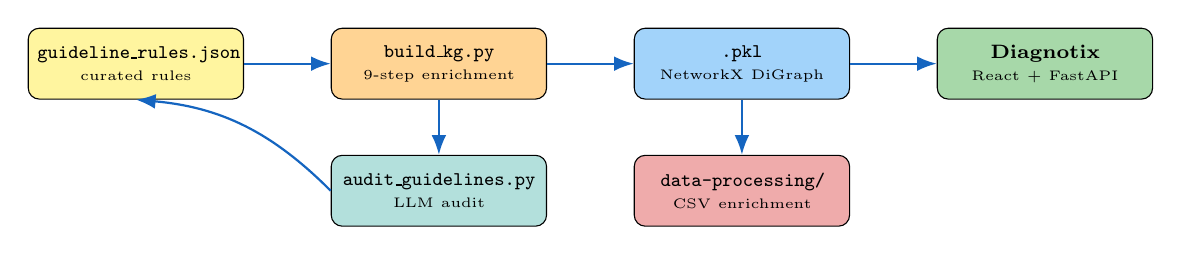
\begin{tikzpicture}[
    node distance=0.7cm and 1.1cm,
    box/.style={draw, rounded corners, fill=lightgray,
                text width=2.5cm, align=center, minimum height=0.9cm,
                font=\scriptsize},
    arr/.style={-{Latex[length=2.5mm]}, thick, color=midblue},
  ]
    \node[box, fill=riskfactor!70] (json)
      {\texttt{guideline\_rules.json}\\{\tiny curated rules}};

    \node[box, fill=vital!60, right=of json] (build)
      {\texttt{build\_kg.py}\\{\tiny 9-step enrichment}};

    \node[box, fill=condition!60, right=of build] (pkl)
      {\texttt{.pkl}\\{\tiny NetworkX DiGraph}};

    \node[box, fill=testcol!70, right=of pkl] (diagnotix)
      {\textbf{Diagnotix}\\{\tiny React + FastAPI}};

    \node[box, fill=symptom!60, below=of pkl] (pipe)
      {\texttt{data-processing/}\\{\tiny CSV enrichment}};

    \node[box, fill=attribute!60, below=of build] (audit)
      {\texttt{audit\_guidelines.py}\\{\tiny LLM audit}};

    \draw[arr] (json)         -- (build);
    \draw[arr] (build)        -- (pkl);
    \draw[arr] (pkl)          -- (diagnotix);
    \draw[arr] (pkl)          -- (pipe);
    \draw[arr] (build.south)  -- (audit.north);
    \draw[arr] (audit.west)   to[bend right=20] (json.south);
  \end{tikzpicture}

  \vspace{0.4em}
  \small
  Rules are iteratively audited and revised until satisfactory, then
  \texttt{build\_kg.py} serialises the final graph. The \texttt{.pkl}
  powers \textbf{Diagnotix} for dynamic expansion and
  \texttt{data-processing/} for patient CSV enrichment.
\end{frame}

% =============================================================================
\section{Knowledge Graph Construction}
% =============================================================================

\begin{frame}[fragile]{Source of Truth: \texttt{guideline\_rules.json}}
  Each of the 45 rules encodes a single clinical assertion:

  \vspace{0.3em}
  \begin{center}
    \texttt{raw\_symptom} \;\(\longrightarrow\)\; \texttt{condition} \;\(\longrightarrow\)\; \texttt{test}
  \end{center}

  \vspace{0.3em}
  \begin{columns}[T]
    \begin{column}{0.48\textwidth}
      \begin{exampleblock}{Example rule (JSON)}
        \begin{lstlisting}[language={}]
{
  "raw_symptom": "chest pain",
  "node_type": "Symptom",
  "condition": "Acute MI",
  "test": "ECG",
  "source": "AHA/ACC"
}
        \end{lstlisting}
      \end{exampleblock}
    \end{column}
    \begin{column}{0.48\textwidth}
      \begin{block}{Rule fields}
        \small
        \begin{tabular}{@{}ll@{}}
          \textbf{Field}      & \textbf{Meaning} \\
          \midrule
          \texttt{raw\_symptom} & Clinical entity \\
          \texttt{node\_type}   & KG category \\
          \texttt{condition}    & Target diagnosis \\
          \texttt{test}         & Recommended test \\
          \texttt{source}       & Guideline body \\
        \end{tabular}
      \end{block}
    \end{column}
  \end{columns}
\end{frame}

\begin{frame}{9-Step Enrichment Pipeline (\texttt{build\_kg.py})}
  \small
  \begin{tabular}{@{}clll@{}}
    \toprule
    \textbf{Step} & \textbf{API / Source} & \textbf{Enriches} & \textbf{Column(s) added} \\
    \midrule
    0 & Static rules          & ---               & base DataFrame \\
    1 & \texttt{GUIDELINE\_URLS} dict & \texttt{(source, test)} & \texttt{url} \\
    2 & EMBL-EBI OLS4 (HP/MONDO/EFO) & \texttt{raw\_symptom} & \texttt{ebi\_code}, \texttt{synonyms} \\
    3 & Infoway FHIR (SNOMED CT CA)  & \texttt{raw\_symptom} & \texttt{infoway\_code} \\
    4 & UMLS REST (LOINC)            & \texttt{test}         & \texttt{loinc\_code} \\
    5 & UMLS REST (ICD-10-CM)        & \texttt{condition}    & \texttt{icd10\_code} \\
    6 & NLM RxNorm + OpenFDA         & \texttt{treatment}    & \texttt{rxcui}, \texttt{adverse\_event} \\
    7 & Europe PMC                   & symptom \(\leftrightarrow\) condition & \texttt{literature\_weight} \\
    8 & Europe PMC                   & condition \(\leftrightarrow\) test & \texttt{test\_literature\_weight} \\
    9 & ClinicalTrials.gov v2        & condition \(\leftrightarrow\) treatment & \texttt{trial\_count} \\
    \bottomrule
  \end{tabular}

  \vspace{0.4em}
  Steps 7--9 attach \textbf{real-world evidence counts} that drive edge-width
  scaling in the HTML visualisation.
\end{frame}

\begin{frame}{Graph Schema}
  \begin{columns}[T]
    \begin{column}{0.44\textwidth}
      \textbf{Primary node types}\\[0.4em]
      \begin{tabular}{@{}ll@{}}
        \nodebox{symptom!80}{Symptom}     & \texttt{Symptom:} \\[2pt]
        \nodebox{condition!80}{Condition} & \texttt{Condition:} \\[2pt]
        \nodebox{testcol!80}{Test}        & \texttt{Test:} \\
      \end{tabular}

      \vspace{0.6em}
      \textbf{Secondary node types}\\[0.4em]
      \begin{tabular}{@{}ll@{}}
        \nodebox{vital!80}{Vital}            & \texttt{Vital:} \\[2pt]
        \nodebox{demo!70}{Demographic}       & \texttt{Demographic:} \\[2pt]
        \nodebox{riskfactor!80}{Risk Factor} & \texttt{Risk Factor:} \\[2pt]
        \nodebox{moi!70}{MOI}                & \texttt{MOI:} \\[2pt]
        \nodebox{attribute!80}{Attribute}    & \texttt{Attribute:} \\[2pt]
        \nodebox{treatment!80}{Treatment}    & \texttt{Treatment:} \\
      \end{tabular}
    \end{column}
    \begin{column}{0.53\textwidth}
      \textbf{Edge types}\\[0.4em]
      \begin{tabular}{@{}ll@{}}
        \texttt{INDICATES\_CONDITION}     & entity \(\to\) condition \\[2pt]
        \texttt{REQUIRES\_TEST}           & condition \(\to\) test \\[2pt]
        \texttt{DIRECTLY\_INDICATES\_TEST}& entity \(\to\) test \\[2pt]
        \texttt{RECOMMENDS\_TREATMENT}    & condition \(\to\) drug \\
      \end{tabular}

      \vspace{0.8em}
      \textbf{Edge metadata on every edge:}
      \begin{itemize}
        \item \texttt{source} --- guideline body (AHA/ACC, ACR, \ldots)
        \item \texttt{source\_url} --- citable DOI or page URL
        \item evidence weight (literature / trial count)
      \end{itemize}
    \end{column}
  \end{columns}
\end{frame}

% =============================================================================
\section{Guideline Audit Pipeline}
% =============================================================================

\begin{frame}{\texttt{audit\_guidelines.py} --- Three-Pass Audit}
  \textbf{Problem:} LLM-generated triage rules can be fabricated, vague, or
  misattributed. The audit pipeline retroactively cleans
  \texttt{guideline\_rules.json} before it enters the graph.

  \vspace{0.6em}
  \begin{block}{Pass 1 --- Schema \& source pre-filter}
    Drops rules with missing required fields or unrecognised guideline bodies
    (allowlist of 33 organisations: AHA/ACC, ACR, NICE, CTAS, ESC, \ldots).
  \end{block}

  \begin{block}{Pass 2 --- LLM clinical verification (per pathway)}
    Rules are grouped by diagnostic test and sent to an Azure OpenAI reviewer.
    The LLM checks: (1) source accuracy, (2) clinical plausibility,
    (3) condition specificity. Only rules that pass all three are kept.
    \emph{When in doubt, remove --- false negatives are safer.}
  \end{block}

  \begin{block}{Pass 3 --- Name normalisation}
    \texttt{condition} $\to$ ICD-10-CM canonical description (NLM API).\quad
    \texttt{raw\_symptom} $\to$ HP/MONDO canonical label (EBI OLS4 API).
    Original string kept when no high-confidence match is found.
  \end{block}
\end{frame}


% =============================================================================
\section{Data Processing Pipeline}
% =============================================================================

\begin{frame}{Data Processing Pipeline --- Two-Phase Overview}
  \textbf{Goal:} ingest a real patient CSV and enrich every diagnosis with
  KG-derived diagnostic tests.

  \vspace{0.5em}
  \begin{columns}[T]
    \begin{column}{0.48\textwidth}
      \begin{block}{Phase 1 --- Extract candidate tests}
        \texttt{csv\_extract\_potential\_test.py}\\[0.3em]
        Reads all unique diagnoses from the \texttt{dx} column and asks
        Azure OpenAI to identify the standard diagnostic test(s) for each.
        Writes \texttt{diagnoses\_to\_tests\_graph\_data.json}.
      \end{block}
    \end{column}
    \begin{column}{0.48\textwidth}
      \begin{block}{Phase 2 --- Expand graph \& map patients}
        \texttt{kg\_enrichment\_pipeline.py}\\[0.3em]
        Adds any new test pathways to the KG, rebuilds the graph with full
        ontology enrichment, then maps every diagnosis back to a condition
        node and its recommended tests.
      \end{block}
    \end{column}
  \end{columns}

  \vspace{0.5em}
  \begin{block}{Standalone mapping (graph already current)}
    \texttt{csv\_mapping.py} --- skips graph expansion; semantically maps a
    new patient CSV against the existing PKL via Azure OpenAI.
  \end{block}
\end{frame}

\begin{frame}[fragile]{Phase 1 --- \texttt{csv\_extract\_potential\_test.py}}
  \begin{columns}[T]
    \begin{column}{0.52\textwidth}
      \textbf{Input:} patient CSV with a \texttt{dx} (diagnosis) column.\\[0.5em]
      \textbf{Steps:}
      \begin{enumerate}
        \item Collect all unique diagnosis strings from \texttt{dx}.
        \item Batch them (default 20 per call) to Azure OpenAI.
        \item LLM consolidates variant spellings into canonical test names
              suitable as KG node labels\\
              (e.g.\ all variants of ``US Appendix'' $\to$
              \texttt{"Appendix Ultrasound"}).
        \item Write \texttt{diagnoses\_to\_tests\_graph\_data.json}.
      \end{enumerate}
    \end{column}
    \begin{column}{0.44\textwidth}
      \begin{exampleblock}{Output (per diagnosis)}
        \begin{lstlisting}[language={}]
{
  "diagnosis":
    "Acute Appendicitis",
  "diagnostic_tests": [
    "Appendix Ultrasound",
    "Complete Blood Count"
  ]
}
        \end{lstlisting}
      \end{exampleblock}
    \end{column}
  \end{columns}
\end{frame}

\begin{frame}{Phase 2 --- \texttt{kg\_enrichment\_pipeline.py}}
  \footnotesize
  \begin{tabular}{@{}cp{9.5cm}@{}}
    \toprule
    \textbf{Step} & \textbf{Action} \\
    \midrule
    1  & Read \texttt{diagnoses\_to\_tests\_graph\_data.json}; collect unique test names. \\
    1b & \emph{(Optional)} LLM ranks candidates by clinical importance; keep top \(N\) via \texttt{--top-x}. \\
    2  & For each new test, call Azure OpenAI to generate 8--15 triage rules grounded in clinical guidelines. \\
    3  & Append new rules to \texttt{guideline\_rules.json} (tests already present are skipped). \\
    4  & Rebuild the PKL via \texttt{build\_kg.generate\_knowledge\_graph()} --- full multi-ontology enrichment. \\
    5  & Semantically map every \texttt{dx} value to a graph condition node; write enriched CSV. \\
    \bottomrule
  \end{tabular}

  \vspace{0.4em}
  \begin{columns}[T]
    \begin{column}{0.48\textwidth}
      \begin{alertblock}{Checkpoint / resume}
        Step 5 writes a sidecar checkpoint after every LLM call.
        Interrupted runs resume from where they left off.
      \end{alertblock}
    \end{column}
    \begin{column}{0.48\textwidth}
      \begin{block}{Output columns added to CSV}
        \texttt{matched\_graph\_condition}\\{\small best-matching \texttt{Condition:} node}\\[0.3em]
        \texttt{potential\_tests}\\{\small tests linked via \texttt{REQUIRES\_TEST}}
      \end{block}
    \end{column}
  \end{columns}
\end{frame}

% =============================================================================
\section{Diagnotix Web Application}
% =============================================================================

\begin{frame}[fragile]{Diagnotix --- Dynamic Knowledge Graph Builder}
  \begin{columns}[T]
    \begin{column}{0.52\textwidth}
      \textbf{Full-stack web application (FastAPI + React)}

      \begin{itemize}
        \item Enter any diagnostic test name; the LLM extracts
              8--15 evidence-based triage rules automatically.
        \item Generated rules are validated and audited via
              \texttt{audit\_guidelines.py} before being committed
              to the graph.
        \item Validated rules are appended to
              \texttt{guideline\_rules.json} and the full ontology
              enrichment pipeline re-runs.
        \item Every expansion is auditable: the response reports
              new rule count and updated node/edge totals.
      \end{itemize}
    \end{column}
    \begin{column}{0.45\textwidth}
      \begin{block}{\texttt{POST /api/kg/expand}}
        \begin{lstlisting}[language={}]
{ "diagnostic_test": "CT Head" }

-> {
  "new_rules_added": 11,
  "nodes": 98,
  "edges": 247
}
        \end{lstlisting}
      \end{block}
      \begin{block}{Stack}
        \small
        Backend: FastAPI + Uvicorn\\
        Frontend: React 19 + TypeScript + Vite\\
        LLM: Claude (Anthropic API)
      \end{block}
    \end{column}
  \end{columns}
\end{frame}

% =============================================================================
\section{Summary}
% =============================================================================

\begin{frame}{Summary}
  \small
  \begin{columns}[T]
    \begin{column}{0.48\textwidth}
      \textbf{What we built}
      \begin{itemize}
        \item An expandable knowledge graph spanning 5 clinical
              pathways, grounded in evidence-based guidelines.
        \item 9-step ontology enrichment pipeline (SNOMED, LOINC,
              ICD-10, HP/MONDO, RxNorm, Europe PMC,
              ClinicalTrials.gov).
        \item LLM-powered audit pipeline to ensure rule accuracy
              and source attribution.
        \item Two-phase data processing pipeline for back-mapping
              patient diagnoses to recommended diagnostic tests.
      \end{itemize}
    \end{column}
    \begin{column}{0.48\textwidth}
      \textbf{Future work}
      \begin{itemize}
        \item Continuously improve the audit pipeline to maintain
              knowledge graph accuracy over time.
        \item Integration with the SickKids database
              (where feasible).
        \item Extend from \emph{back prediction} (diagnosis
              $\to$ test) to \emph{front prediction} --- using
              patient vitals at triage to recommend tests,
              grounded in the knowledge graph.
        \item Expert clinician verification of the constructed
              knowledge graph.
      \end{itemize}
    \end{column}
  \end{columns}
\end{frame}

% ─────────────────────────────────────────────────────────────────────────────
\end{document}
